\chapter{myc2d.h,myc.h Documentation}
\ifsingle
\maketitle
\fi
\chaptermeta[draft][2025-07-15]

\section{Introduction}
‘MYC’ stands for the Mixed Young’s Centered scheme, introduced by Scardovelli et al. \cite{2003_Scardovelli}. It is used to compute the interface normal vector $\mathbf{n}$ at a given cell, based on the volume fraction $c$ in the current cell and its neighboring cells (9 cells in 2D and 27 cells in 3D).

In the following sections, I will first introduce the basic concept of representing an interface with a linear function, followed by the algorithm that enables the mixed scheme to determine the normal direction in 2D cases. This will then be extended to the 3D scenario.

\section{2D scenario}
\subsection{Linear Representation of the Interface}

Consider an interfacial cell on a 2D plane, as shown in figure \ref{fig:myc-2Dlinear}. Let the normal direction of the interface be denoted by $\mathbf{n} = (n_x, n_y)$. It is straightforward to show that the interface can be represented by the linear equation
\begin{equation}\label{equ:myc-original}
  n_x X + n_y Y = \alpha,
\end{equation}
where $\alpha$ is a constant that determines the position of the interface.

\begin{figure}[H]
    \centering
    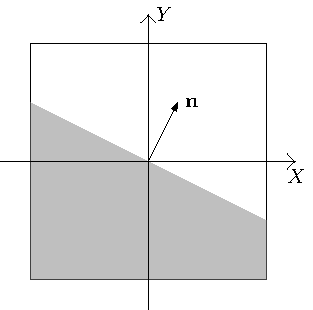
\includegraphics[height=5.5cm]{./image/myc-h-and-myc2d-h/2Dlinear-face.pdf}
    \caption{Linear representation of the interface, with normal direction $\mathbf{n} = (n_x, n_y)$.}
    \label{fig:myc-2Dlinear}
\end{figure}

This equation indicates that the linear interface within a cell is fully characterized once the triplet $(n_x, n_y, \alpha)$ is known.

If we treat $Y$ as a function of $X$, the equation takes the slope-intercept form
\begin{equation}\label{equ:myc-centered}
  sign(n_y)Y = -\frac{n_x}{|n_y|} X + \frac{\alpha}{|n_y|} = m_y X + b_y,
\end{equation}
where $m_y = -\frac{n_x}{|n_y|}$ and $b_y = \frac{\alpha}{|n_y|}$.

Similarly, $X$ can be expressed as a function of $Y$, with slope $m_x = -\frac{n_y}{|n_x|}$. The normal direction obtained from equation \ref{equ:myc-centered} can thus be written in the form $(-m_x,, \text{sign}(n_y))$ (or equivalently, $(\text{sign}(n_x),, -m_y)$). This form is derived by transforming equation \ref{equ:myc-centered} back into the original form of the interface representation, as shown in equation \ref{equ:myc-original}.

With the interface representation clarified, we now introduce the centered scheme, Young’s scheme, and finally the mixed scheme. As will be shown, the centered scheme estimates the interface normal direction through the form of equation \ref{equ:myc-centered}, while Young’s scheme directly computes the normal vector $(n_x, n_y)$.
\subsection{Centered columns scheme}\label{sec:myc-centered}

For the linear equation \ref{equ:myc-centered}, the most straightforward way to compute the slope is by selecting an arbitrary pair of points on the line, denoted as $(X_1, Y_1)$ and $(X_2, Y_2)$, and calculating  
\begin{equation}
  m_x = \frac{Y_2 - Y_1}{X_2 - X_1}.
\end{equation}  
The centered columns scheme adopts the same idea but operates under discrete conditions. This naturally raises several questions:  
\begin{enumerate}
  \item Given a value of $X$, how can we determine the corresponding output $Y$ in a discrete setting?
  \item Since there are two slope estimates, which one should be selected?
\end{enumerate}

\begin{figure}[H]
    \centering
    \begin{subfigure}[t]{0.45\textwidth}
        \centering
        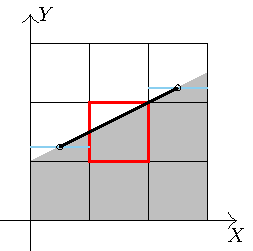
\includegraphics[height=5.5cm]{./image/myc-h-and-myc2d-h/centered-a.pdf}
        \subcaption{}
        \label{fig:myc-centered-a}
    \end{subfigure}
    \begin{subfigure}[t]{0.45\textwidth}
        \centering
        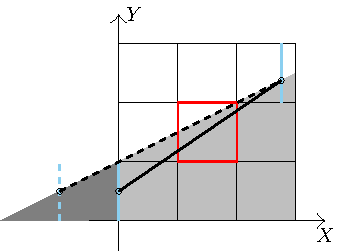
\includegraphics[height=5.5cm]{./image/myc-h-and-myc2d-h/centered-b.pdf}
        \subcaption{}
        \label{fig:myc-centered-b}
    \end{subfigure}
    \caption{Sketch of the computation process for the centered scheme. The red cell highlights the current cell where the interfacial slope is being computed. The blue lines represent the summation of volume fractions across columns, and the black solid line shows the resulting slope obtained by the centered scheme. In figure (a), the scheme accurately captures the interface when it spans across opposite boundaries. By contrast, figure (b) presents the same scenario but from a complementary perspective. The result reveals a significant discrepancy between the computed and actual slopes. Note that the dashed and solid lines are intentionally reversed to facilitate comparison with the true slope of the interface.}
    \label{fig:myc-centered}
\end{figure}

Figure \ref{fig:myc-centered-a} illustrates the first question by showing how the centered scheme computes the interfacial slope. Similar to the height function method described in the \texttt{heights.h} documentation, the value of $Y$ at each column is approximated by summing the volume fractions $c$ of three adjacent cells aligned along the same $X$ coordinate. Once two neighboring values (marked as empty circles) are obtained, the slope at the current cell (highlighted in red) is computed using a centered finite difference. The result is indicated by the solid black line.

Let the current cell be denoted by index $(0, 0)$. The slope in figure~\ref{fig:myc-centered-a} is then given by:
\begin{equation}\label{equ:myc-dcentered}
m_x = \frac{1}{2} \left(\sum_{j=-1}^{1} c_{1,j} - \sum_{j=-1}^{1} c_{-1,j} \right)
\end{equation}

Since $m_x = -\frac{n_y}{|n_x|}$, it follows that $\text{sign}(n_x) = -\text{sign}(m_x)$, and similarly, $\text{sign}(n_y) = -\text{sign}(m_y)$. This dual representation for the same interface raises the second question: which of the two directional estimates gives the more accurate result?

Figure \ref{fig:myc-centered-b} presents the same scenario but treats $Y$ as the independent variable and $X$ as the dependent output. In this case, the slope computed by the centered scheme deviates significantly from the true interface, as part of the left column (shown in dark gray) is omitted. For a perfectly linear interface, the centered scheme yields accurate results only when the interface intersects the left and right boundaries of the current cell. However, when the interface crosses adjacent boundaries (e.g., left and top) or spans the top and bottom boundaries, the accuracy deteriorates due to partial volume loss, as illustrated in figure~\ref{fig:myc-centered-b}. In other words, the smaller the absolute value of the slope, the more accurate the estimate \cite{2007_Aulisa}.

Based on this observation, the normal direction is chosen as $(-m_x, sign(m_y))$ when $|m_y| > |m_x|$, and as $(sign(m_x), -m_y)$ otherwise.

\subsection{Young's Scheme}

\begin{figure}[H]
  \centering
  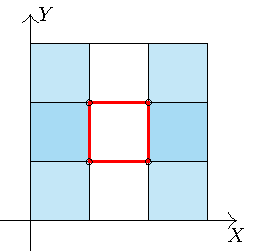
\includegraphics[height=5.5cm]{./image/myc-h-and-myc2d-h/Youngs.pdf}
  \caption{Illustration of Young's scheme. The interface normal is obtained by averaging the normals at four cell corners, indicated by empty circles. Blue shading marks the cells involved in the final algebraic expression, with dark blue showing overlaps.}
  \label{fig:myc-young}
\end{figure}

Young's scheme estimates the interface normal vector $\mathbf{n}$ by averaging the normals computed at four cell corners. As shown in figure \ref{fig:myc-young}, the normal at each corner is evaluated using central differences of the surrounding cell values. For example, considering the target cell with index $(0,0)$, the $x$-component of the normal at corner $(1/2, 1/2)$ is given by
\begin{equation}
  n_{x,(1/2,1/2)} = \frac{1}{2\Delta}\left(c_{1,1} + c_{1,0} - c_{0,1} - c_{0,0}\right)
\end{equation}
The average $x$-component of the normal over all four corners is then computed as
\begin{equation}
  n_x = \frac{1}{4} \left(n_{x,(1/2,1/2)} + n_{x,(-1/2,1/2)} + n_{x,(1/2,-1/2)} + n_{x,(-1/2,-1/2)} \right)
\end{equation}

Alternatively, a more compact expression for $n_x$ can be obtained by directly summing the contributions from relevant cells:
\begin{equation}
  n_x = \frac{1}{8} \left(C_1 - C_{-1}\right)
\end{equation}
where
\begin{equation}\label{equ:myc-youngs}
  C_1 = c_{1,1} + 2c_{1,0} + c_{1,-1}, \quad C_{-1} = c_{-1,1} + 2c_{-1,0} + c_{-1,-1}
\end{equation}
as indicated by the blue regions in figure \ref{fig:myc-young}. The same procedure applies for computing $n_y$. Note that the coefficient $\frac{1}{8}$ may be omitted or replaced, provided both components of $\mathbf{n}$ are scaled consistently.

\subsection{Mixed Young's and Centered scheme}\label{sec:myc-myc}
In the previous two sections, two normals—$\mathbf{n}_Y$ and $\mathbf{n}_C$—were computed separately, with the subscripts denoting the respective schemes. The MYC scheme unifies these by introducing a criterion to select the more accurate normal. In summary, the criterion favors the normal with the larger absolute value. While $\mathbf{n}_C$ is already normalized, $\mathbf{n}_Y$ must be normalized consistently—based on the selected $\mathbf{n}_C$—to enable a fair comparison.

Consider the example shown in figure~\ref{fig:myc-MYC}, where the interface has a slope of $3/4$. For simplicity, the cut-cell areas are labeled locally. Although the interface intersects adjacent cell boundaries, the omitted area (shaded in dark gray) under the current frame is significantly smaller than in the alternative case, suggesting that the resulting normal is more accurate—specifically, $|n_{C,x}| = \frac{35}{48}$. However, the normal obtained using Young’s scheme is $|n_{Y,x}| = \frac{25}{35}$, which is not only favored by the MYC criterion due to its larger magnitude, but also closer to the exact value, making it in fact more accurate than the centered scheme in this case. This improvement stems from the averaging process in Young’s scheme, which reduces the influence of the omitted area that would otherwise tend to reduce the magnitude of the normal.


\begin{figure}[H]
  \centering
  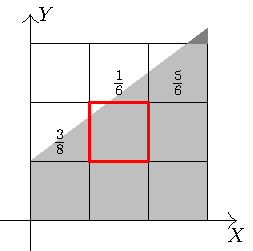
\includegraphics[height=5.5cm]{./image/myc-h-and-myc2d-h/MYC.pdf}
  \caption{An example illustrating the difference between the two schemes. The red cell denotes the target interfacial cell, with the interface having a slope of $3/4$. For simplicity, the cut-cell areas are labeled locally within each intersected cell.}
  \label{fig:myc-MYC}
\end{figure}

\subsection{\func{myc} (2D version)}
\subsubsection{Parameters}
\begin{center}
  \begin{tabular}{|c|c|c|c|c|}
    \hline
    Name & Data type & Status & Option/Default & Representation (before/after)\\[0.5ex]
    \hline\hline
    \para{point} & Point & unchanged & compulsory & index $(x,y)$\\
    \hline
    \para{c} & scalar & unchanged & compulsory & $c$\\
    \hline
  \end{tabular}
\end{center}

\begin{codesection}{subsubsection}{Program Workflow}
\codecomment{
  \textbf{Starting Point}\\
  \para{ix}: flag for normal selection in Centered Scheme;\\ 
  \para{c\_t,c\_b,c\_r,c\_l}: volume summation of four columns;\\
  \para{mx0,my0}:normal components obtained by Centered scheme;\para{mx1,my1}: normal components obtained by Young's; \para{mm1,mm2} swap value.
}

\begin{minted}{cpp}
    coord mycs (Point point, scalar c)
  {
    int ix;
    double c_t,c_b,c_r,c_l;
    double mx0,my0,mx1,my1,mm1,mm2;
\end{minted}

\codearrow

\codecomment{
  \textbf{Centered Scheme Computation}\\
  To facilitate equation \ref{equ:myc-dcentered}, note here \para{mx0}=$-m_x$, \para{my0}=$-m_y$
}

\begin{minted}{cpp}
    c_t = c[-1,1] + c[0,1] + c[1,1];
    c_b = c[-1,-1] + c[0,-1] + c[1,-1];
    c_r = c[1,-1] + c[1,0] + c[1,1];
    c_l = c[-1,-1] + c[-1,0] + c[-1,1];

    mx0 = 0.5*(c_l - c_r);
    my0 = 0.5*(c_b - c_t);
\end{minted}

\codearrow

\codecomment{
  \textbf{Centered Scheme Criterion}\\
Select the normal computed by the centered scheme according to the criterion described in section \ref{sec:myc-centered}, and unify the remaining components accordingly. The flag \para{ix} is used to indicate which normal has been selected.
}

\begin{minted}{cpp}
    if (fabs(mx0) <= fabs(my0)) {
      my0 = my0 > 0. ? 1. : -1.;
      ix = 1;
    }
    else {
      mx0 = mx0 > 0. ? 1. : -1.;
      ix = 0;
    }
\end{minted}

\codearrow

\codecomment{
  \textbf{Young's Scheme Computation}\\
Facilitation of equation \ref{equ:myc-youngs}, the \para{NOT\_ZERO} is introduced to avoid division by zero.
}

\begin{minted}{cpp}
    mm1 = c[-1,-1] + 2.0*c[-1,0] + c[-1,1];
    mm2 = c[1,-1] + 2.0*c[1,0] + c[1,1];
    mx1 = mm1 - mm2 + NOT_ZERO;
    mm1 = c[-1,-1] + 2.0*c[0,-1] + c[1,-1];
    mm2 = c[-1,1] + 2.0*c[0,1] + c[1,1];
    my1 = mm1 - mm2 + NOT_ZERO;
\end{minted}

\codearrow

\codecomment{
  \textbf{Mixed Centered and Young's Scheme Criterion}\\
  If \para{ix} = $0$, i.e., the normal $(-m_x, \operatorname{sign}(m_y))$ is selected as the final output of the centered scheme, then $\mathbf{n}Y$ is normalized using the value of $n{y,Y}$—and vice versa. The final output is determined by the criterion described in section \ref{sec:myc-myc} which compares the absolute value of corresponding subcomponent and sored the larger pair in (\para{mx0},\para{my0}).
}

\begin{minted}{cpp}
    if (ix) {
    mm1 = fabs(my1);
    mm1 = fabs(mx1)/mm1;
    if (mm1 > fabs(mx0)) {
      mx0 = mx1;
      my0 = my1;
    }
  }
  else {
    mm1 = fabs(mx1);
    mm1 = fabs(my1)/mm1;
    if (mm1 > fabs(my0)) {
      mx0 = mx1;
      my0 = my1;
    }
  }
\end{minted}

\codearrow

\codecomment{
  \textbf{Final Output}\\
  The final normal, denoted as $\mathbf{n}$, will be normalized such that $n_x + n_y = 1$, to align with the form used in 3D. The reason for this normalization will be explained in the following section.
}

\begin{minted}{cpp}
  mm1 = fabs(mx0) + fabs(my0);
  coord n = {mx0/mm1, my0/mm1, 0};

  return n;
}
\end{minted}

\end{codesection}
  
\printbibliography
